\documentclass[12pt]{article}

\usepackage[utf8]{inputenc}
\usepackage[margin=1in]{geometry}
\renewcommand{\baselinestretch}{1}
\usepackage{indentfirst}

\usepackage{amsmath, amssymb}

\usepackage{hyperref}
\usepackage{cleveref}
\usepackage{graphicx}
\usepackage{float}
\graphicspath{{./figs/}}

\begin{document}

\begin{center}\begin{LARGE}
\textbf{Assignment 3: Results/Description}
\end{LARGE}\end{center}

\section*{Problem 1}

For this problem I have written three programs (\texttt{myEuler},
\texttt{myEulerPC}, and \texttt{myODEINT}) to solve the following problems.
These may be compiled all together with a \texttt{make all} as shown below.

\begin{figure}[H]
    \centering
    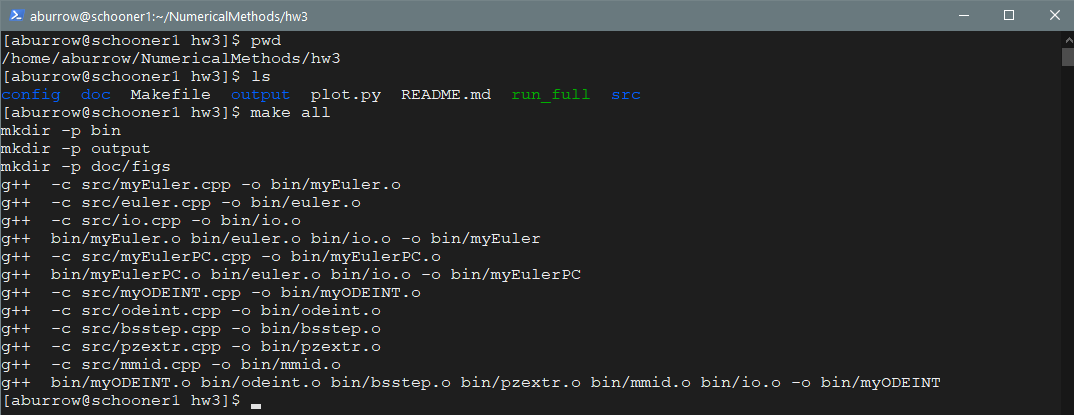
\includegraphics[width=1\textwidth]{compile}
    \label{fig:compile}
\end{figure}

This generates executables \texttt{myEuler}, \texttt{myEulerPC}, and
\texttt{myODEINT} in the ``./bin'' directory, which may be run one at a time.
There is also a \texttt{plot.py} in the root which may be run to generate plots
from the output of the executables. However, to run all these programs at once,
I have included a \texttt{run\_full} bash script that may be executed for more
ease.

For all of these problems, I am solving the equation
$$
\begin{aligned}
\frac{dy}{dx} = f(x, y)
\end{aligned}
$$
for $y(x)$ where $f(x, y) = -\cos x$. We know already that the analytic
solution is $y(x) = -\sin x$, and so I use the boundary condition $y(0) = 0$,
and I solve the equations on the interval $[0, 20\pi]$ (which is 10 cycles of
the periodic function).

\subsection*{(a)}

Below I run the program that demonstrates solving our differential equation
using the Euler method:
\begin{figure}[H]
    \centering
    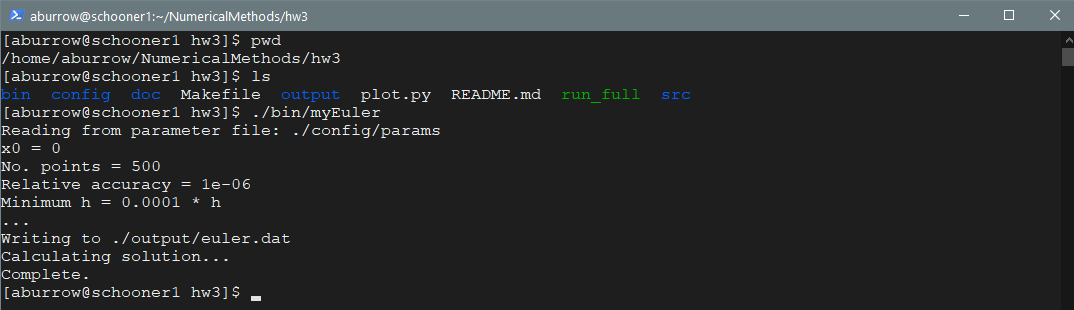
\includegraphics[width=1\textwidth]{myEuler}
    \label{fig:myEuler}
\end{figure}
I solve for 500 points of the solution, and those are plotted in
\autoref{fig:euler}, along with the residual from the analytic solution. We see
that the general trend of the analytic solution is represented by the
calculated solution. Looking at the residuals, they are on the order of
$10^{-1}$, and they are actually asymmetric, so that there is only negative
residual for this solution. Because of this, we see that the solution seems
shifted down and to the right, so that the amplitudes are well described by
the calculated solution.
\begin{figure}[ht]
    \centering
    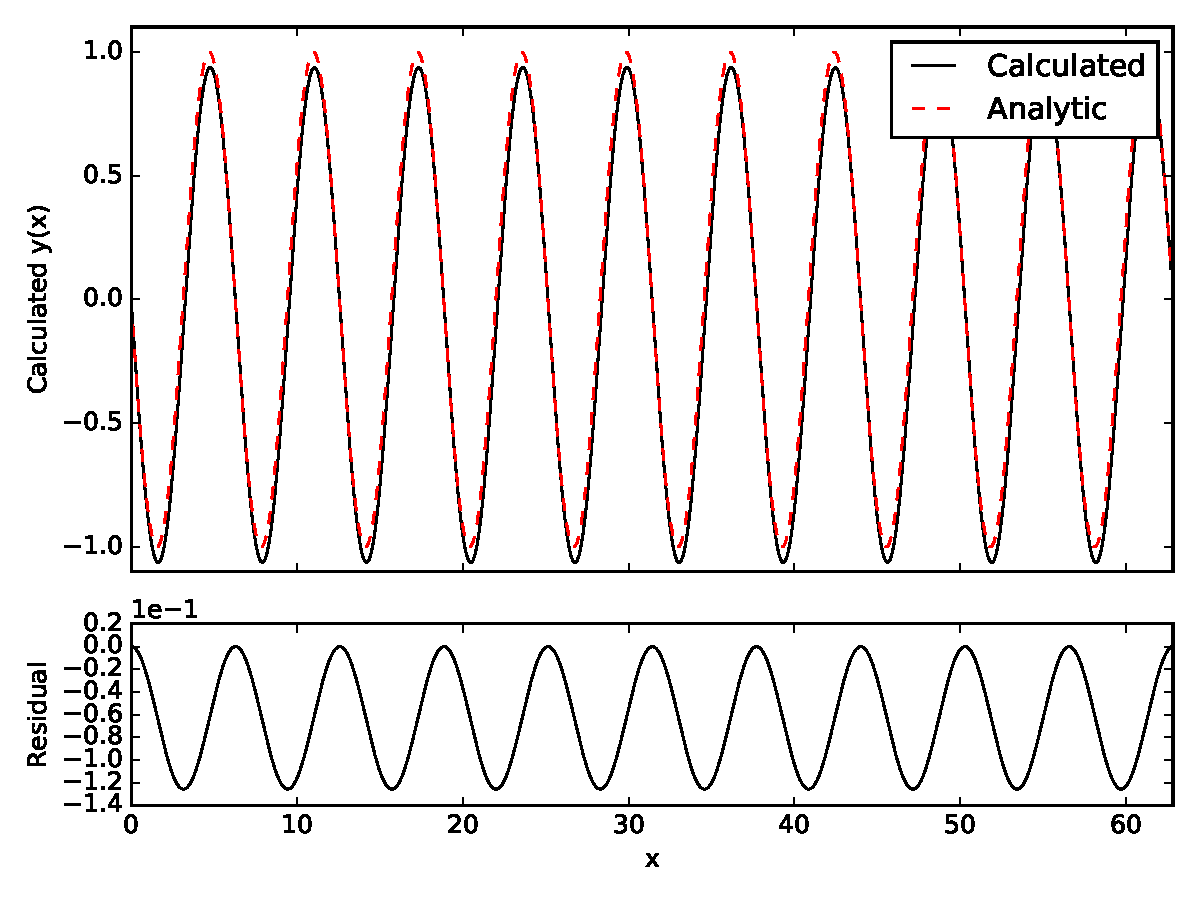
\includegraphics[width=0.9\textwidth]{euler}
    \caption{Solution using the Euler method.}
    \label{fig:euler}
\end{figure}

\subsection*{(b)}

Below I run the program that demonstrates solving our differential equation
using the Euler predictor-corrector method:
\begin{figure}[H]
    \centering
    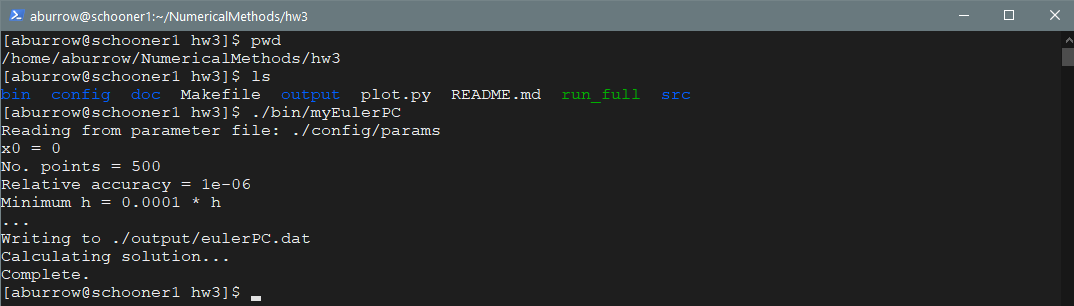
\includegraphics[width=1\textwidth]{myEulerPC}
    \label{fig:myEulerPC}
\end{figure}
Again the solution is found at 500 points, which is shown in
\autoref{fig:eulerPC}. It is clearly a much better fit from the top panel,
however the residuals explain this by showing error on order of $10^{-3}$. The
residuals are also symmetric and for this case they are greatest at the extrema
of the solution.
\begin{figure}[ht]
    \centering
    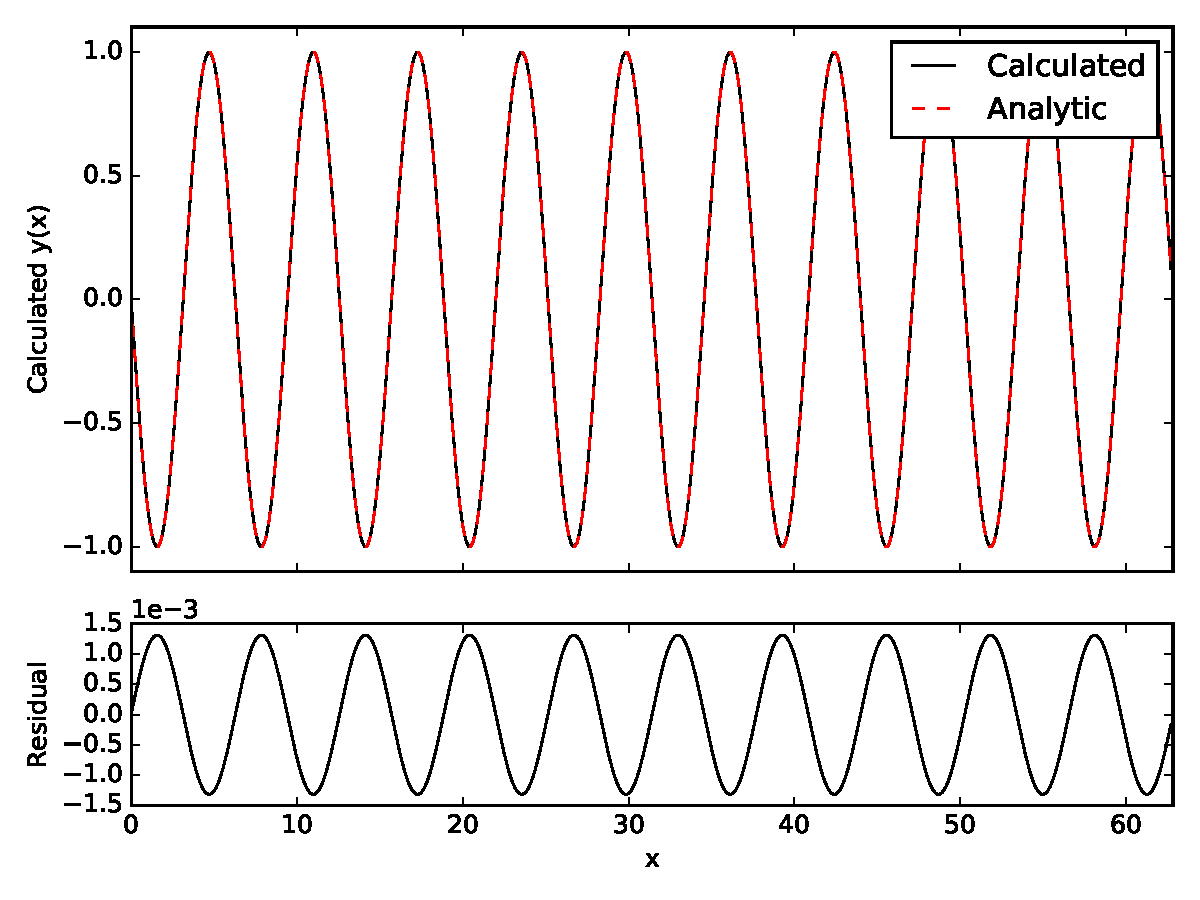
\includegraphics[width=0.9\textwidth]{eulerPC}
    \caption{Solution using the Euler predictor-corrector method.}
    \label{fig:eulerPC}
\end{figure}

\subsection*{(c)}

Finally I run the program that demonstrates solving our differential equation
using the Numerical Recipes' ODEINT function with the Bulirsch-Shoer algorithm
below:
\begin{figure}[H]
    \centering
    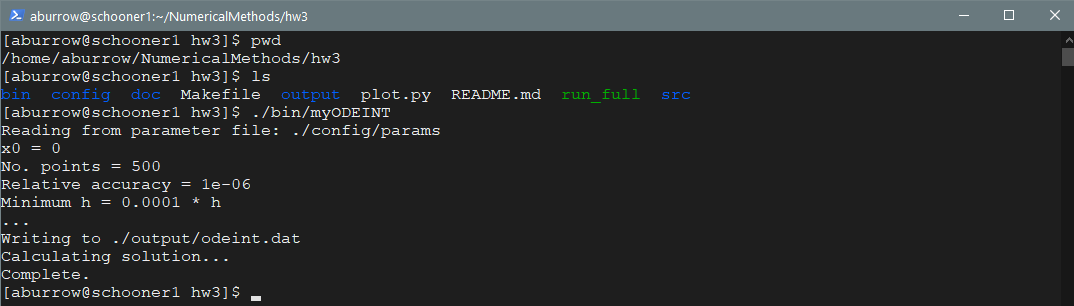
\includegraphics[width=1\textwidth]{myODEINT}
    \label{fig:myODEINT}
\end{figure}
To achieve the solution, I use a relative accuracy of $10^{-6}$ and allowed a
minimum $h$ value of $10^{-4}$ times the initial $h$. The function was applied
to each of the 499 intervals (to get 500 points of the solution), and the
initial $h$ was $1 / 10$ of the interval size. The solution is given in
\autoref{fig:odeint}. Again the top panel shows that the solution fits well
with the analytic solution. The residuals, however, are extremely small
($\sim10^{-11}$!) compared to the previous two methods. The residuals are
asymmetric, and the greatest deviation is seen in the troughs of the solution.
\begin{figure}[ht]
    \centering
    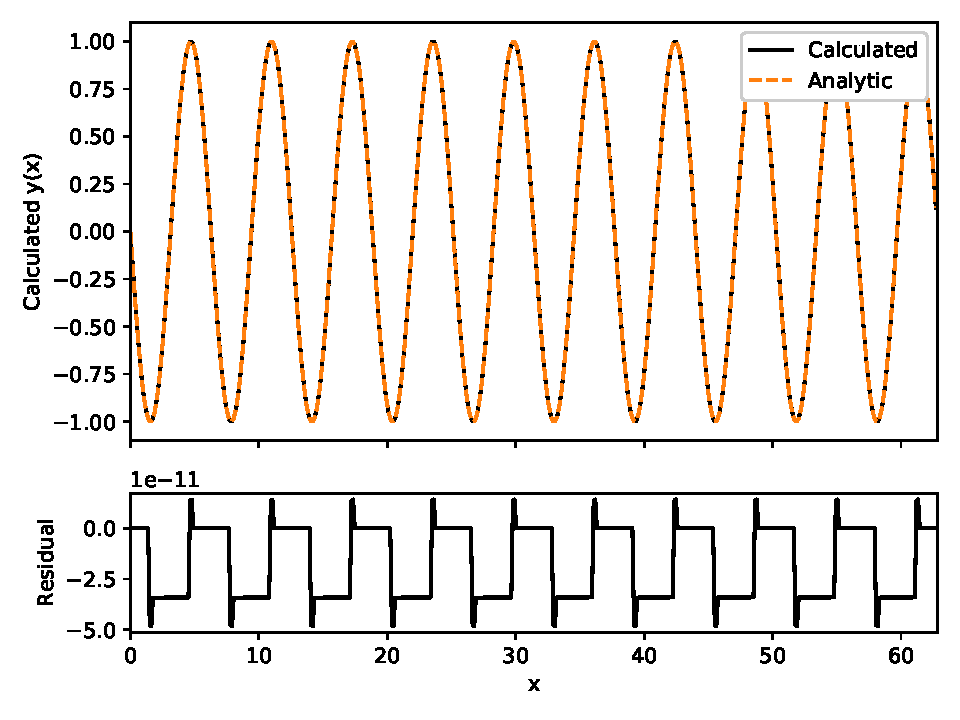
\includegraphics[width=0.9\textwidth]{odeint}
    \caption{Solution using the Numerical Recipes ODEINT (BS) method.}
    \label{fig:odeint}
\end{figure}

\subsection*{(d)}

From the results in parts (a)-(c), we can immediately conclude that the most
representative solution comes from the ODEINT method, as it is orders of
magintude more accurate through the entire solution interval. This is of course
because there is more that goes into this method, such as a level of tolerance
that is used for comparison as well as the extra functionality.

In terms of simplicity, the easiest to code are definitely the first two
methods. Therefore if one wanted to do this from scratch with little hassle,
the best method may be to use the Euler predictor-corrector method, as it still
has the possibility of achieving a solution within an order of $10^{-3}$
(residuals).

\end{document}
